\section{Wicklungsschema Übung 4}
\begin{center}
    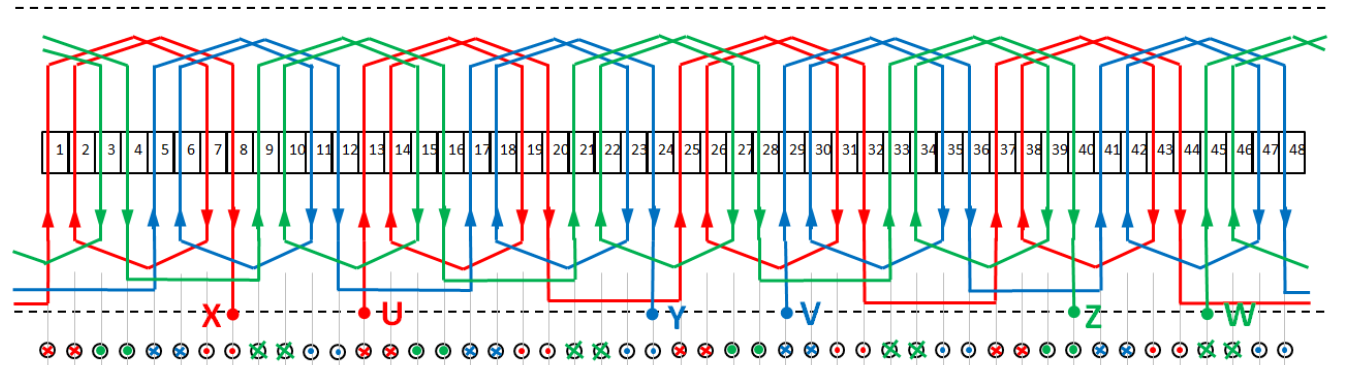
\includegraphics[width = 15cm]{images/Wicklungsschema}\newline
    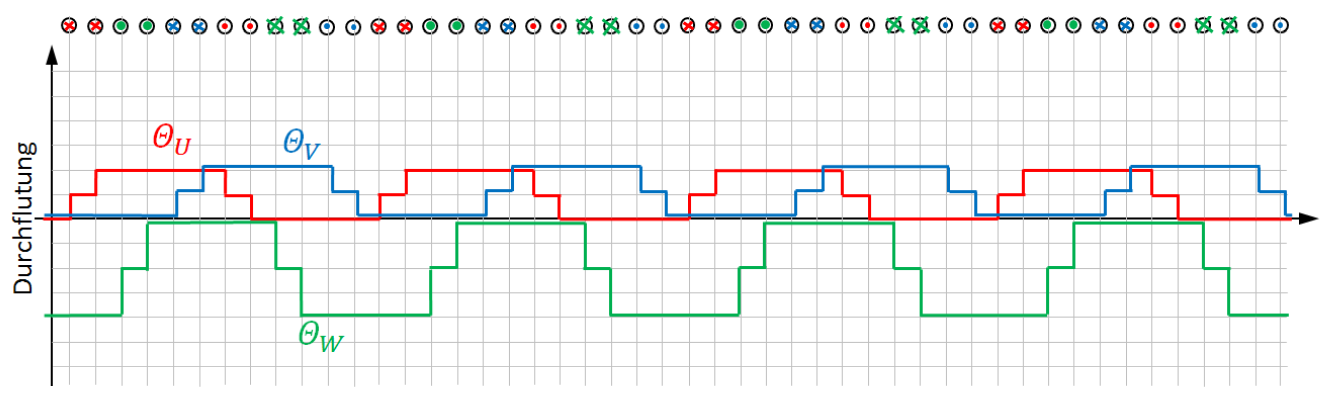
\includegraphics[width = 15cm]{images/Durchflutung3} \newline
    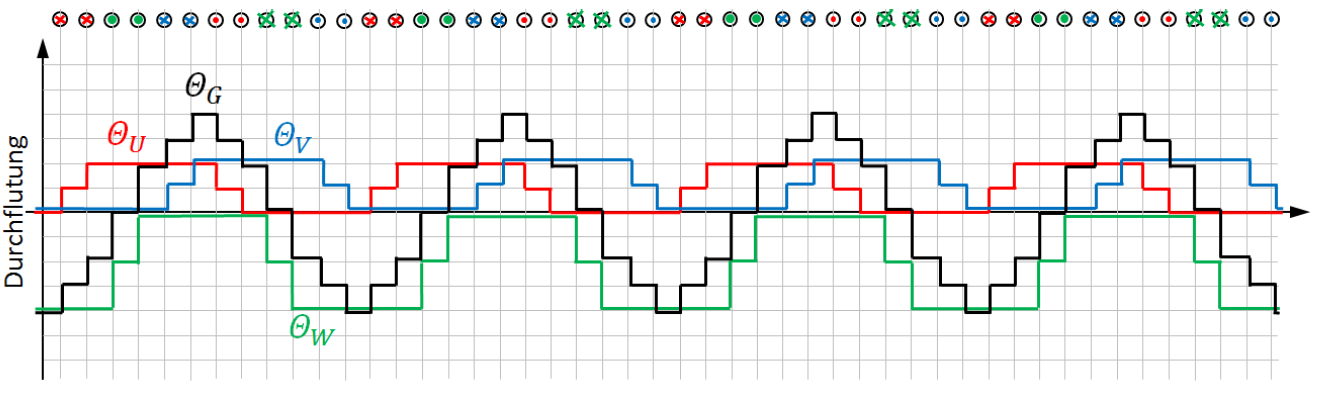
\includegraphics[width = 15cm]{images/Durchflutung4} \newline
\end{center}
\vspace{-1cm}
\subsection{Beispiel}
    \begin{minipage}{0.5\linewidth}	
        $ "\,8-polig "  \rightarrow  Polpaarzahl \; p = 4   \rightarrow  Polzahl \;2p = 8$\newline
        Statornuten N = 48  \newline
        Strangzahl m = 3 (Anz Phase)\newline
        Statornutzahl pro Phasenband $q = \frac{N}{2p \cdot m}= \frac{48}{8 \cdot 3}=2 $\newline
    \end{minipage}
    \begin{minipage}{0.3\linewidth}
        $i_{L1} = Real\{\underline{I_{L1}}\} = 0.5\cdot I_0$ \newline \newline
        $i_{L2} = Real\{\underline{I_{L2}}\} = 0.5\cdot I_0$ \newline \newline
        $i_{L3} = Real\{\underline{I_{L3}}\} = -1.0\cdot I_0$ 
    \end{minipage}
    \begin{minipage}{0.3\linewidth}
    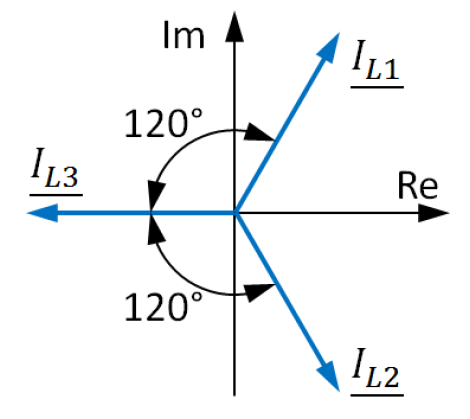
\includegraphics[scale = 0.3]{images/StromdreieckAGS}
\end{minipage}
\vspace{-1cm}
\subsection{Wichtige Formeln}
\renewcommand{\arraystretch}{0.8}
\begin{tabular}{|C{0.3\textwidth}|P{0.3\textwidth}|P{0.3\textwidth}|}
    \hline
    \textbf{Drehzahl n} &
    \[n = 60\cdot \dfrac{f}{p}\] &
    \vspace{0.1cm}n - Drehzahl [n] = $\dfrac{1}{min}$ \newline 
    f - Frequenz \newline
    p - Polpaarzahl 
    \\ \hline
    \textbf{Polpaarzahl p}&
    \[ p= 60\cdot \dfrac{f}{n} \]&
    p=floor(p) bei ASM
    \\ \hline 
    \textbf{Nutzahl N} &
    \[ N = 2p\cdot q\cdot m\] &
    2p - Polzahl \newline 
    q - Nutzahl pro Phasenband \newline
    m - Strangzahl pro Phase 
    \\ \hline  						 
\end{tabular}
\clearpage